\documentclass[crop=false]{standalone}
% --- ПРЕАМБУЛА ДЛЯ ПОДДЕРЖКИ РУССКОГО ЯЗЫКА И МАТЕМАТИКИ ---
\usepackage[T2A]{fontenc}
\usepackage[utf8]{inputenc}
\usepackage[russian]{babel}
\usepackage{amsmath}
\usepackage{geometry}
\usepackage{amssymb}
\usepackage{graphicx}
\usepackage{float}
\usepackage{import}
\geometry{a4paper, top=2cm, bottom=2cm, left=2cm, right=2cm}
\newcommand{\sidecomment}[1]{\marginpar{\raggedright\scriptsize\itshape #1}}
\newcommand{\iu}{\mathrm{i}}

\newcommand{\Def}{%
    \text{Def}%
    \hspace{-0.85em}% Сдвиг назад ровно на середину (подберите под шрифт)
    \raisebox{0.1ex}{/}% Черта
    \hspace{1em}% Возврат к концу слова + небольшой отступ
}

\renewcommand{\Re}{\operatorname{Re}}
\renewcommand{\Im}{\operatorname{Im}}

\ifstandalone
    \newcommand{\lecturebreak}{} % В отдельном файле лекции разрыв не нужен
\else
    \newcommand{\lecturebreak}{\clearpage} % В полной книге - начинаем с новой страницы
\fi

\newcounter{lecturenumber} % Создаем счетчик для нумерации лекций
\newcommand{\lecture}[2]{
    \lecturebreak
    \refstepcounter{lecturenumber} % Увеличиваем счетчик на 1
    \par\vspace{2em}\noindent % Отступ сверху и убираем абзацный отступ
    {\Large\bfseries % Делаем заголовок крупным и жирным
    Лекция \thelecturenumber: #1 % Выводим "Лекция N: Тема"
    \hfill % Растягиваем пробел, чтобы дата была справа
    \large\textit{#2}} % Выводим дату курсивом
    \par\vspace{1em} % Небольшой отступ снизу
    \addcontentsline{toc}{section}{Лекция \thelecturenumber: #1} % Добавляем в оглавление
    \par
}

\newcommand{\TwoCols}[2]{%
  \par\noindent % Начать с новой строки без отступа
  \begin{minipage}[t]{0.48\textwidth}
    #1
  \end{minipage}% <-- Важный '%' для удаления пробела
  \hfill % Растягивающийся пробел между колонками
  \begin{minipage}[t]{0.48\textwidth}
    #2
  \end{minipage}% <-- Важный '%' для удаления пробела
  \par%
}

\pagestyle{plain} % Включаем нумерацию страниц\
\begin{document}
\lecture{}{27.01}
\subsection{Вид матрицы направляющих косинусов}
Известно из Линейной алгебры, Сергей Алексеевич привёл следующую цепочку
\[\lambda_{2,3} = \cos \varphi \pm \iu \sin \varphi \to \bar p \pm \iu \bar q, \]
\[A(\bar p \pm \iu \bar q) = (\cos \varphi \pm \iu \sin \varphi)(\bar p \pm \iu \bar q) = \bar p \cos \varphi - \bar q \sin \varphi  \pm (\iu \bar p \sin \varphi + \iu \bar q \cos \varphi)\]
\begin{theorem}[Теорема Эйлера о конечном повороте]
    Произвольное перемещение абсолютно твёрдого тела с неподвижной точкой предстваляет собой поворот вокруг некоторой оси, проходящей через эту точку
\end{theorem}
\subsection{Сложение поворотов}
\begin{figure}[H]
    \centering
    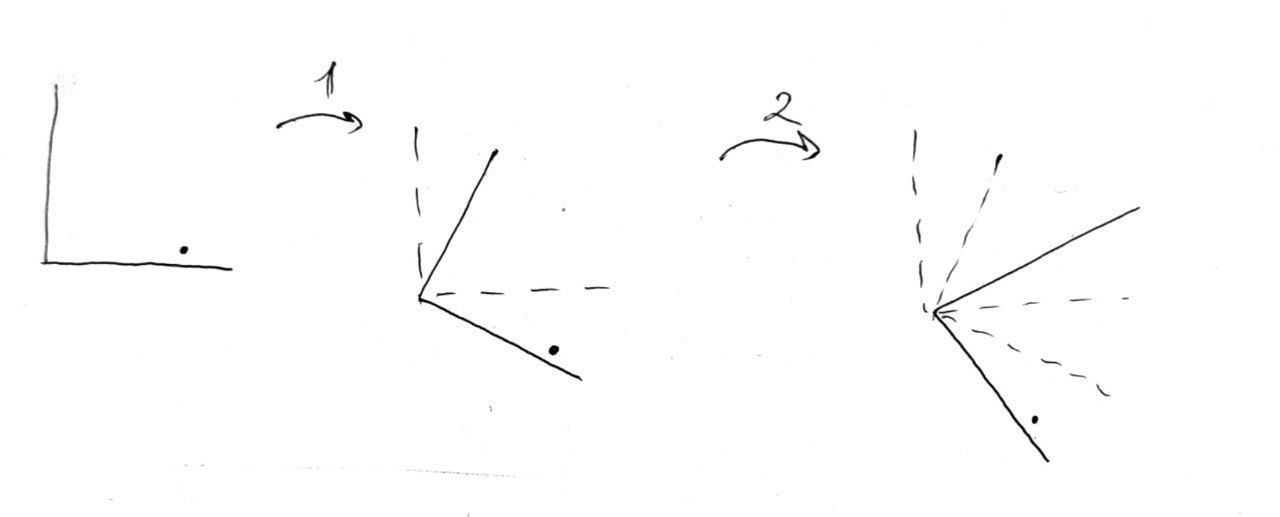
\includegraphics[width=0.5\textwidth]{СложениеПоворотов.jpg}
    \caption{}
    \label{fig:myimage} % Sets a label for cross-referencing
\end{figure}
\TwoCols{
Активная точка зрения(все матрицы в исходной ск):
\[
\begin{cases} 
    \bar r_1 = A_1 \bar r_0 \\ 
    \bar r_2 = A_2 \bar r_1 
\end{cases} \implies \bar r_2 = A_2 A_1 \bar r_0 = A \bar r_0
\]
}
{
Пассивная точка зрения(каждая последующая в предыдущей ск):
\[
\begin{cases} \bar r_1' = \bar r_0 \\ \bar r_1 = A_1 \bar r_1'
\end{cases} \qquad \bar r_2 = A_1 \bar r_2' = A_1 A_2' \bar r_1' = A_1 A_2' \bar r_0\]
}
\section{Повороты во времени}
\[A(t) \qquad \bar r = A(t) \bar r_0\]
\[\bar v = \frac{d \bar r}{d t} = \dot {\bar r} = \overset{\textstyle \cdot}{(A \bar r_0)} = \dot A \bar r_0 = \dot A A^{T} \bar r = \Omega \bar r\]
\begin{proof}
     \[\qquad E = A A^T \qquad O = \dot A A^T + A \dot A^T \qquad \dot A A^T = -(\dot A A^T)^T \qquad \Omega = - \Omega^T\]
\end{proof}
    \[
    \begin{aligned}
\Omega \bar r = \begin{pmatrix}
    0 & \omega_{12} & \omega_{13} \\
    -\omega_{12} & 0 & \omega_{23} \\
    -\omega_{13} & -\omega_{23} & 0
\end{pmatrix} \begin{pmatrix}
    x \\ y \\ z
\end{pmatrix} &= \begin{pmatrix}
    \omega_{12} y + \omega_{13} z \\
    -\omega_{12} x + \omega_{23} z \\
    -\omega_{13} x - \omega{23} y
\end{pmatrix} \\
&= \begin{vmatrix}
    \bar e_1 & \bar e_2 & \bar e_3 \\
    -\omega_{23} & \omega_{13} & -\omega_{12} \\
    x & y & z
\end{vmatrix} = \Bigl[\{-\omega_{23} , \omega_{13} , -\omega_{12}\},  \{x,y,z\}\Bigr]
\end{aligned}
\]
\Def Угловая скорость – вектор $\bar \omega = \begin{pmatrix}
    \omega_x, \omega_y, \omega_z
\end{pmatrix}^T$, где
\[\omega_x = -\omega_{23} \qquad \omega_y = \omega_{13} \qquad \omega_z = - \omega_{12}\]
\keypoint Вывод формулы эйлера для распределения скоростей твёрдого тела
\begin{figure}[H]
    \centering
    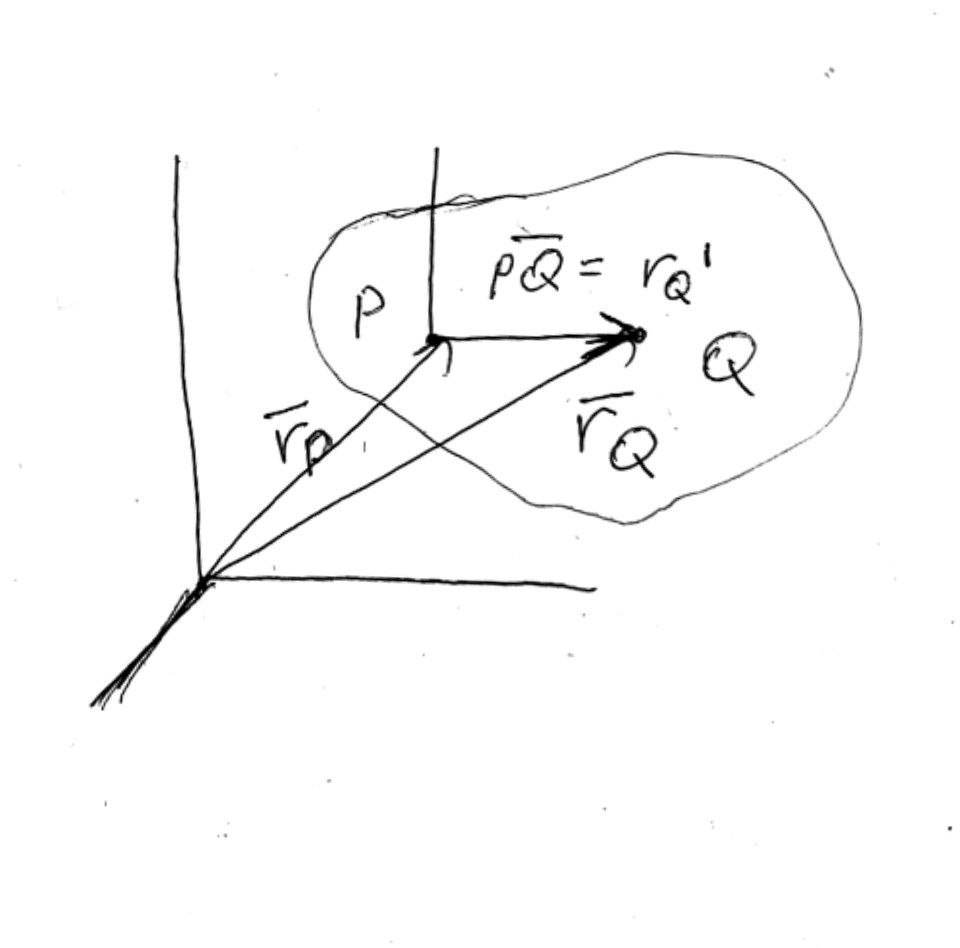
\includegraphics[width=0.5\textwidth]{ФормулаЭйлера.jpg}
    \caption{}
    \label{fig:myimage} 
\end{figure}
\[\bar v = \bar \omega \times \bar r \]
\[\bar v_Q' = \bar \omega \times \bar r'_Q\]
\[\bar r_a' = \bar r_Q - \bar r_P = \overline{PQ}\]
\[\bar v_Q' = \bar v_Q - \bar v_P\]
Тогда
\[\bar v_Q - \bar v_P = \bar \omega \times (\bar r_Q - \bar r_P)\] 
\[\boxed{\bar v_Q = \bar v_P + \bar \omega \times \overline{PQ}}\]
Следствия: %fixme как оформлять следствия(я всегда делал в кружочках номера)
\begin{enumerate}
\item проекции скоростей двух точек твёрдого тела на оси соединяющие их равны
%fixme картинка 
\[(\bar v_Q , \overline{PQ}) = (\bar v_P , \overline{PQ})\]
\begin{proof}
    $(\bar v_Q , \overline{PQ}) = (\bar v_P , \overline{PQ}) + (\bar \omega, \overline{PQ}, \overline{PQ})$
\end{proof}
\item
Скорости двух точек твёрдого тела вполне определяют скорости точек твёрдого тела, лежащих на прямой, соединяющей данные 
\begin{proof}
    \[\bar v_A = \bar v_O + \bar \omega \times \overline{OA} \qquad \bar v_B = \bar v_O + \bar \omega \times \overline{OB}\]
    \[\bar v_A - \bar v_B = \bar \omega \times \overline{BA} \qquad \bar v_c = \bar v_B + \bar \omega \times \overline{BC}\]
    \[A, B, C \in l \iff \overline{BA} \| \overline{BC} \iff \exists! \lambda: \overline{BC} = \lambda \overline{BA}\]
    \[\bar v_c = \bar v_B + \lambda \bar \omega \times \overline{BA}\]
\end{proof}
\item
Скорость трёх точек твердого тела, не лежащих на одной прямой, вполне определяют скорость в любой точке твёрдого тела

\item
Если скорость точки твёрдого тела равна нулю, то это тело либо покоится либо совершает мгновенное вращение вокруг оси, проходящей через эту точку
\end{enumerate}
\keypoint 
Угловое ускорение:
\[\dot{\bar \omega} := \bar \varepsilon \qquad \dot {\bar r} = \bar \omega \times \bar r\]
\[\bar w = \dot{\bar v} = \dot{\bar \omega} \times \bar r + \bar \omega \times \dot{\bar r} = \bar \varepsilon \times \bar r + \bar \omega \times (\bar \omega \times \bar r)\]
Формула Ривальса
\[
\boxed{
\bar w_Q = \bar w_P + \bar \varepsilon \times \overline{PQ} + \bar \omega \times (\bar \omega \times \overline{PQ})
}\]
\end{document}